\documentclass[11pt,a4paper]{article}
\usepackage[utf8]{inputenc}
\usepackage[english]{babel}
\usepackage[T1]{fontenc}
\usepackage{amsmath, amssymb, amsthm}
\usepackage{geometry}
\usepackage{graphicx}
\usepackage{hyperref}

\geometry{margin=2.5cm}
\title{Temporal Matching for Decentralized Ridesharing Systems}
\author{
  André de Palma\thanks{Email: \href{mailto:andre.de-palma@cyu.fr}{andre.de-palma@cyu.fr}} \\
  Viery Naoussi\thanks{Corresponding author. Email: \href{mailto:naoussiviery237@gmail.com}{naoussiviery237@gmail.com}} \\
  \textit{Thema, Cergy Paris Université}
}

\date{April 15, 2026}

\begin{document}
\baselineskip=16pt
\maketitle

\begin{abstract}
This paper develops a dynamic temporal matching framework for decentralized ridesharing systems in which passengers and drivers are matched sequentially over time under evolving spatial and temporal constraints. The model incorporates dynamic vehicle capacities, schedule delay costs, and user compatibility, while accounting for decentralized individual decision-making. Matching outcomes are determined using an adapted Gale–Shapley deferred acceptance mechanism to ensure stability of assignments over a discretized time horizon. The framework proposes to integrate dynamic ridesharing, temporal assignment, and stable matching into a unified equilibrium model adaptable to large transportation networks.
\end{abstract}

\textbf{Key words:} Dynamic ridesharing; Stable matching; Gale–Shapley mechanism; Temporal assignment; Decentralized equilibrium; Transportation networks.

\section{Introduction}
\indent Urban transportation systems face increasing pressure from congestion, parking scarcity, and rising mobility costs. At the same time, public transportation remains costly to operate in low-density areas despite continued network expansion. Yet private car use (of kilometers travelled) in countries such as France and Switzerland has remained broadly stable over the past decade. This apparent contradiction highlights the persistent attractiveness of individual car travel despite growing economic and environmental concerns (see Small et al., 2024). One possible avenue for improving transport efficiency without reducing mobility is to increase vehicle occupancy rates. In this perspective, dynamic ridesharing constitutes an attractive mechanism for better utilizing existing vehicle capacity. This paper seeks to contribute to that objective.

Dynamic ridesharing
 (or ride-matching) has emerged as a promising approach to improving transportation efficiency through real-time matching passengers and drivers. Unlike traditional pre-arranged carpooling systems, dynamic ridesharing requires assignments to be determined continuously as users enter the platform, under evolving spatial and temporal constraints. This creates a complex allocation problem involving route compatibility, vehicle capacities, travel-time uncertainty, and heterogeneous user preferences. We also treat compatibility between drivers and passengers, and among passengers, as a key explanatory variable. This type of sorting is already implemented in a basic form in BlaBlaCar services. The theoretical foundations of the matching approach are based on the optimal transport model (for a clear introduction, see Galichon, 2018).

Most existing ridesharing models formulate the assignment process as a static optimization problem in which all ride requests and driver availabilities are assumed to be known ex ante over the planning horizon (Agatz et al., 2012; Furuhata et al., 2013). Although this assumption allows for tractable optimization formulations, it fails to capture the sequential arrival of users and the dynamic nature of vehicle occupancy in real-world ridesharing platforms.

To address these limitations, several studies have introduced dynamic ridesharing formulations incorporating real-time requests and rolling-horizon optimization procedures (Kleiner et al., 2011; Stiglic et al., 2015). However, most of these approaches remain centralized and assume the existence of a platform operator capable of continuously recomputing socially optimal assignments based on full system information. In practice, such assumptions may be unrealistic when users retain autonomy over their transportation decisions and evaluate alternatives according to individual preferences.

In decentralized environments, passengers select transportation options by minimizing their perceived travel costs while accounting for punctuality constraints, and walking disutility. The relevant equilibrium concept extends beyond global efficiency and requires the consideration of matching stability, that is, the absence of mutually beneficial deviations between passengers and drivers. While matching theory has been extensively applied in economics and market design (Gale and Shapley, 1962; Roth and Sotomayor, 1990), its integration into dynamic ridesharing remains relatively underdeveloped.

This paper proposes a dynamic temporal matching framework for ridesharing in which assignments are explicitly modeled as time-dependent functions over a discretized time horizon. That is, it is a dynamic temporal matching model with sequential arrivals and discrete-time stable assignment. We check that in the same car all occupants are mutually compatible. The framework incorporates sequential passenger arrivals, dynamic vehicle capacities, asymmetric schedule delay costs, walking alternatives, and compatibility constraints between users sharing the same vehicle. Total vehicle capacities are given. Passenger decisions are represented through individual cost minimization, and equilibrium matching is computed using an adapted many-to-one Gale–Shapley deferred acceptance algorithm.

The contribution of this paper is fourfold. First, it provides a formal dynamic representation of the ridesharing assignment problem, accounting explicitly for temporal evolution. Second, it introduces a decentralized equilibrium model combining transportation cost minimization with stable matching principles. Third, it establishes the existence of stable dynamic assignments under standard behavioral and operational assumptions and proposes an implementable matching algorithm. Fourth, it presents preliminary results for a large-scale network.

The remainder of the paper is organized as follows. Section 2 reviews the related literature. Section 3 introduces the formal dynamic ridesharing model. Section 4 presents the analytical definition costs. Section 5 describes the decentralized modeling approach. Section 6 defines the objective of stable matching. Section 7 describes the matching algorithm and stability results. Section 8 presents preliminary results. Section 9 concludes and discusses possible extensions toward multi-hop ridesharing.

\section{Literature Review}

\subsection{Static Optimization Models for Ridesharing}
The ridesharing problem has traditionally been studied as a combinatorial optimization problem closely related to vehicle routing and assignment models. Early formulations treat ridesharing as a static matching problem, in which the objective is to minimize aggregate travel cost subject to route and capacity constraints.

Agatz et al. (2012) provide a comprehensive review of optimization approaches for ridesharing and emphasize that most formulations assume complete information regarding all users before matching takes place. Similarly, Furuhata et al. (2013) survey algorithmic developments in ridesharing systems and highlight the predominance of static bipartite and network-flow formulations used in the literature.

While static approaches offer computational tractability and theoretical clarity, they remain poorly suited for real-time mobility systems where passenger requests and driver availability evolve continuously over time.

Static matching models based on dynamic traffic models (incorporating schedule delay costs) have been investigated by de Palma et al. (2022), for small toy networks. For an introduction to dynamic models in transportation, see Arnott et al. (1993). Simulation results for such dynamic models are presented in de Palma, et al. (2024).

\subsection{Dynamic and Real-Time Ridesharing Models}
To better represent operational ridesharing systems, several authors have developed dynamic formulations incorporating time-dependent arrivals and rolling-horizon optimization.

Kleiner et al. (2011) propose an auction-based framework for dynamic ridesharing in which ride requests are matched through repeated bidding rounds. Their approach demonstrates the feasibility of real-time decentralized allocation but remains focused on short-term assignment efficiency.

Stiglic et al. (2015) extend dynamic ridesharing analysis by introducing meeting points and showing that flexible pickup locations substantially improve system performance. More broadly, dynamic optimization methods generally rely on repeated centralized computation of assignments as new requests appear.

Despite their realism, these models typically assume centralized coordination and perfect platform information, thereby neglecting strategic user behavior and decentralized acceptance decisions.
\newpage
\subsection{Matching Theory and Stability in Transportation Systems}
The concept of stable matching originates from Gale and Shapley (1962), who introduced the deferred acceptance algorithm and established the existence of stable allocations in two-sided matching markets. Their framework was later generalized to many-to-one settings and extensively developed in the market design literature (see, Roth and Sotomayor, 1990).

Stable matching concepts have progressively been introduced into transportation and logistics applications where decentralized agents interact strategically. Ashlagi et al. (2017) show that stability considerations are crucial in dynamic markets characterized by heterogeneous preferences and sequential arrivals.

In ridesharing contexts, stable assignments are particularly relevant because passengers and drivers may reject proposed matches if preferable alternatives exist. However, relatively few studies explicitly model ridesharing as a stable matching problem rather than a centralized optimization problem.


\subsection{Multi-Hop and Transfer-Based Extensions}
A major limitation of most ridesharing models is the assumption that each passenger is matched to a single driver for the entire trip. This single-hop framework restricts feasible matching opportunities and may significantly reduce network efficiency.

Masson et al. (2014) study transportation systems with transfers and demonstrate that allowing intermediate reallocation substantially increases assignment flexibility and service rates. Similar results are observed in multimodal transport literature, where transfer possibilities improve network connectivity but generate significantly greater computational complexity.

Although multi-hop ridesharing appears promising, introducing transfers transforms the assignment problem into a dynamic path-finding problem over temporal networks, requiring considerably more sophisticated and faster algorithms. Preliminary results on multi-hops are presented in Stokkink, et al. (2025) for simple networks.

Despite these advances, the integration of dynamic assignment, decentralized decision-making, and matching stability remains insufficiently explored in the ridesharing literature.

The present paper focuses on the single-hop case as a foundational framework while laying the groundwork for future multi-hop extensions.

\section{The Proposed Dynamic Ridesharing Model}
The modeling approach is dynamic. The assignment (or matching) is defined as a function evolving over time. Figure~\ref{fig:network_instance} illustrates a typical instance of the problem on the Cergy-Pontoise road network, showing the spatial distribution of passengers and drivers at the beginning of an observation period.

\begin{figure}[htbp]
    \centering
    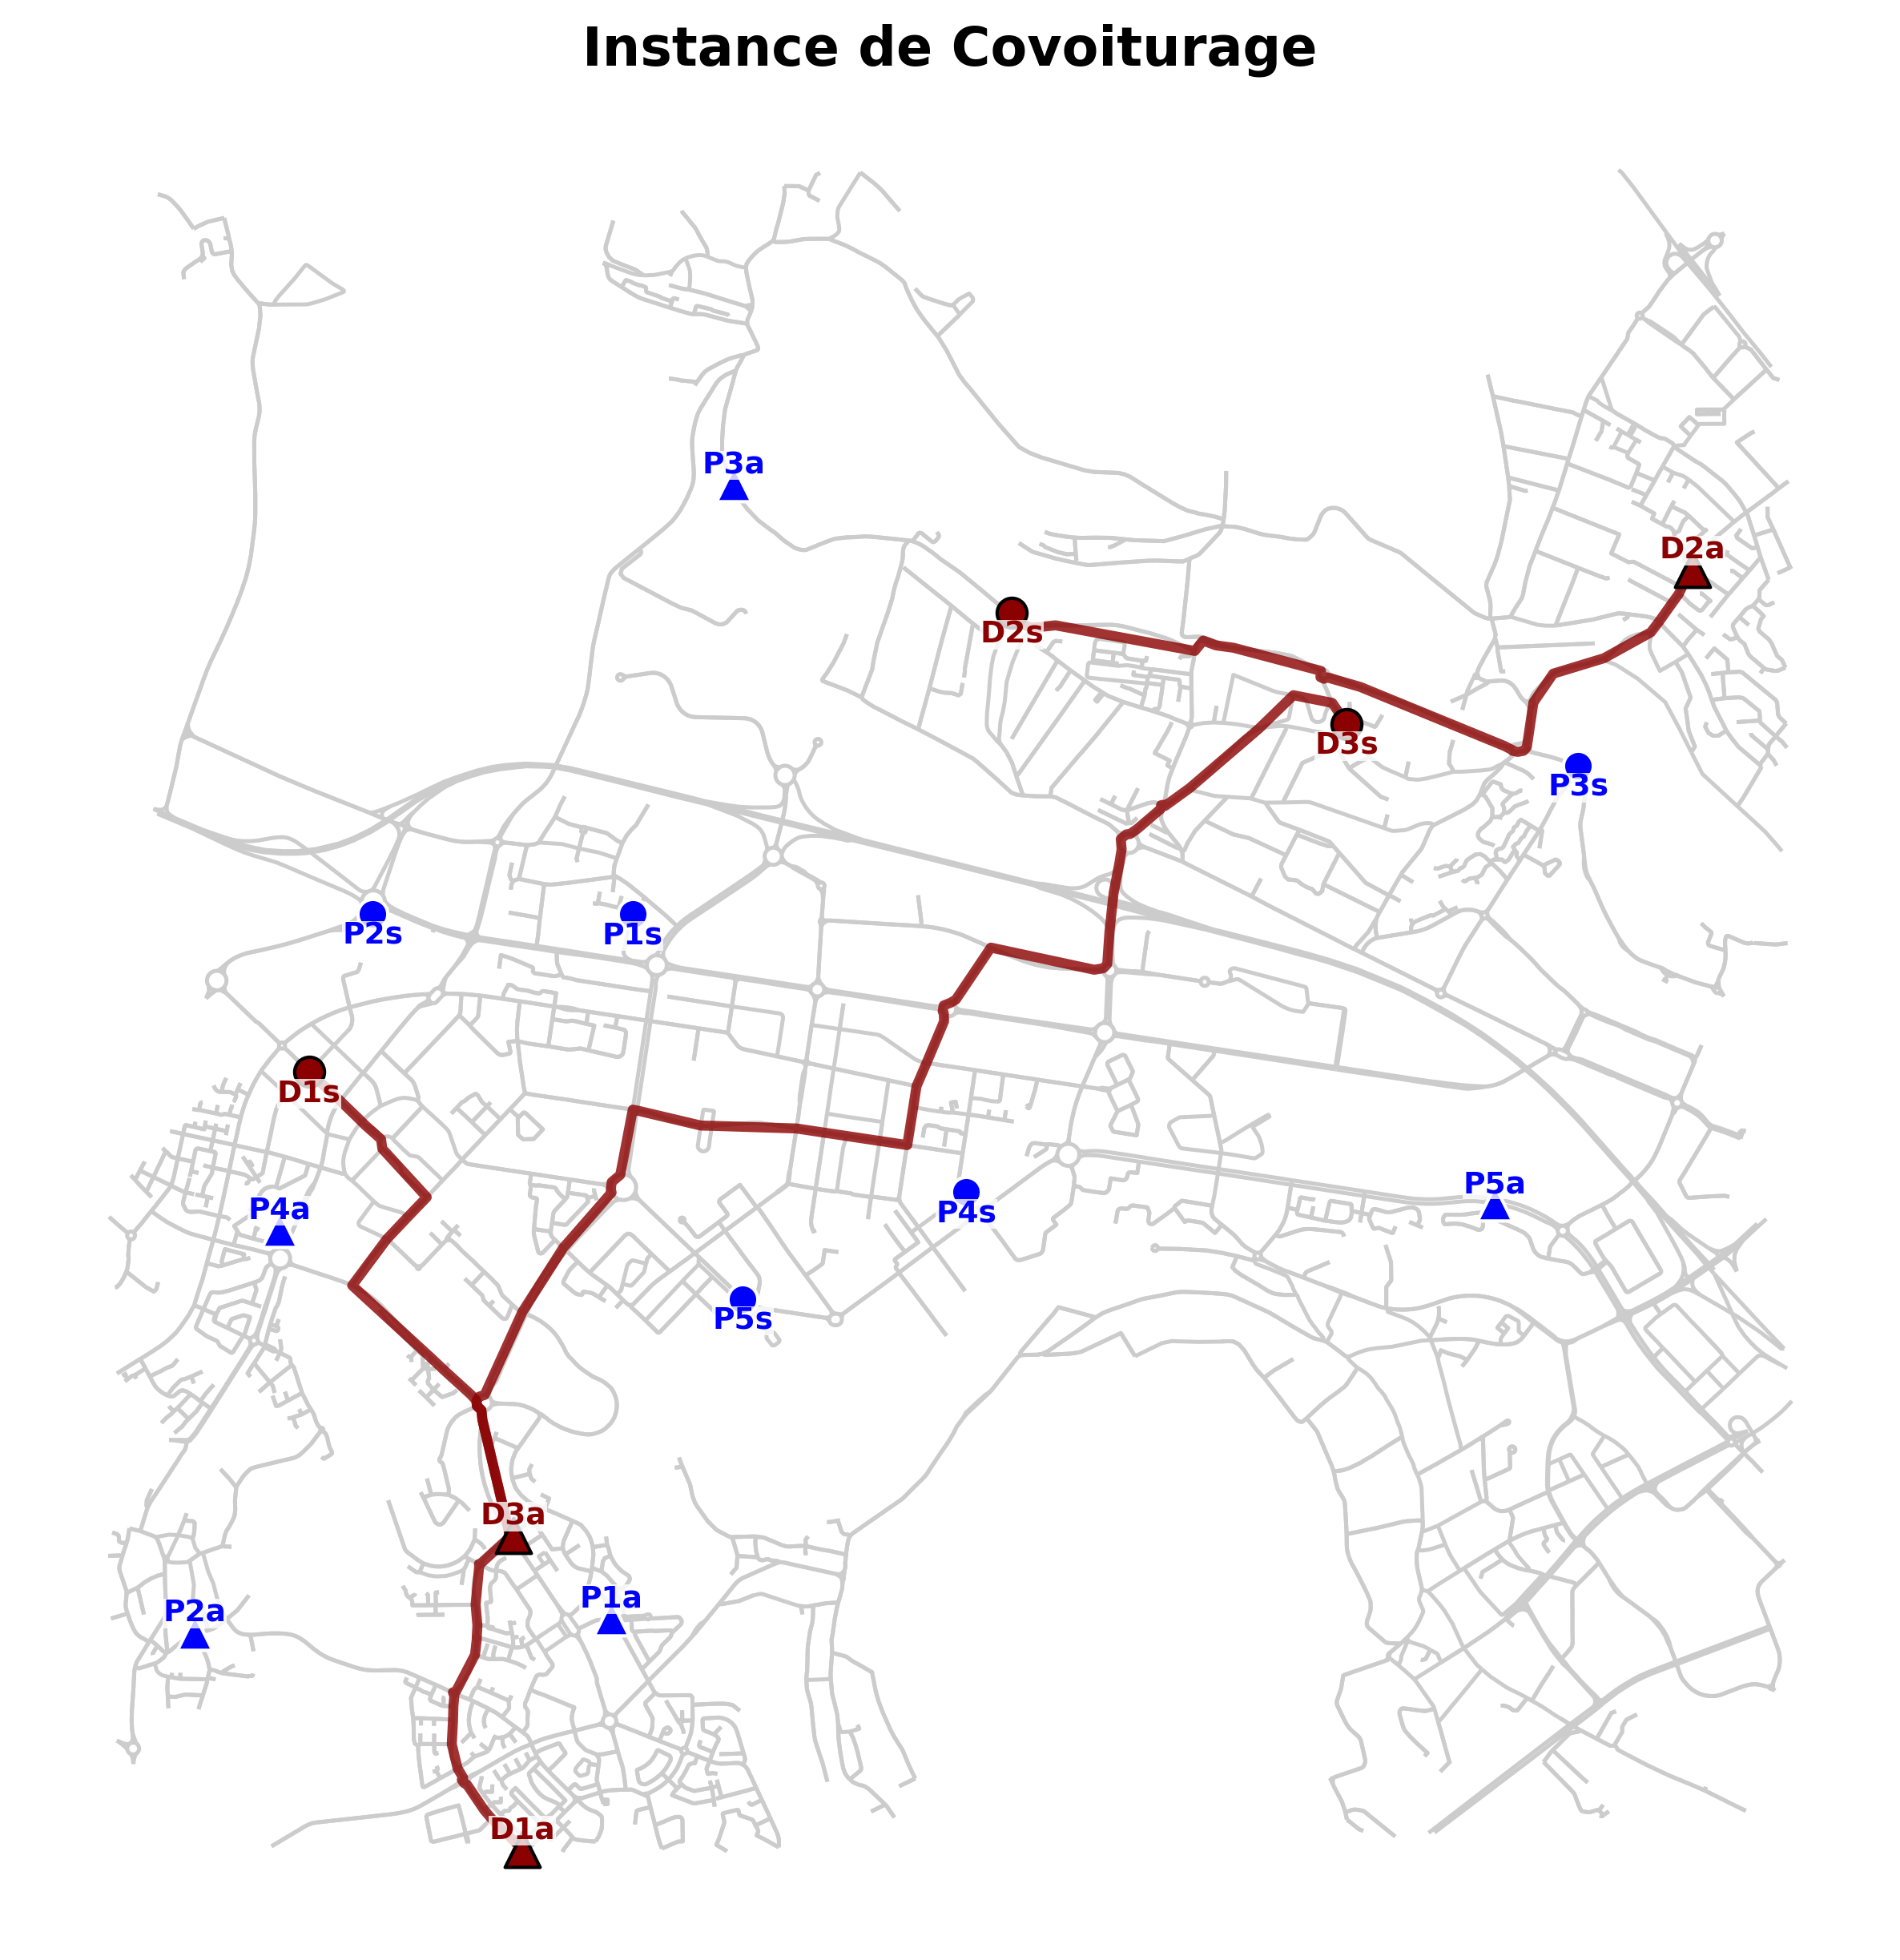
\includegraphics[width=0.8\textwidth, trim={0 0 0 1.2cm}, clip]{map_covoiturage.png}
    \caption{Spatial representation of the road network and agents in Cergy.}
    \label{fig:network_instance}
\end{figure}

In this visualization, blue symbols represent passengers and red symbols represent drivers. Points (circles) indicate the origins of the agents, while triangles represent their respective destinations. The red lines illustrate the predefined fixed routes that each driver follows. Matching is only feasible if a passenger's origin and destination lie within an acceptable distance from these routes, respecting the temporal constraints of both parties.

The following sections formally define the agents and temporal constraints involved in the matching process.

\subsection{Agents and Time Interval}
The problem involves two types of agents:
\begin{itemize}
    \item $P = \{p_1, \dots, p_n\}$, the set of passengers.
    \item $D = \{d_1, \dots, d_k\}$, the set of real drivers.
\end{itemize}
To model the walking alternative, we introduce a set of ``phantom'' vehicles, $F = \{f_1, \dots, f_n\}$, one for each passenger. The extended set of vehicles is denoted by:
\[ D' = D \cup F \]
Matching is performed over a discretized time interval $T$:
\begin{itemize}
    \item Let $t_0$ denote the initial observation time of the problem.
    \item Let $\Delta t$ denote a predefined time step (e.g., 1 minute).
    \item The time interval is then defined as: $T = \{t_0, t_0 + \Delta t, t_0 + 2\Delta t, \dots, t_F\}$, where $t_F$ denotes the final time of the problem.
\end{itemize}
By convention, all temporal variables defined in this model ($t^h_j, t^*_j, t^{max\_pickup}_{d_i}$, etc.) belong to $T$, while durations (denoted $\Delta t$) are assumed to be multiples of the time step.

\subsection{Temporal Definitions}
For each passenger $p_j$, we define the following temporal variables:
\begin{itemize}
    \item $t^h_j$: departure time of passenger $p_j$ from home.
    \item $t^m_{i,j}$: meeting time between passenger $p_j$ and driver $d_i$.
    \item $tt^{wo}_{i,j}$: walking time required for passenger $p_j$ to reach the pickup point with driver $d_i$ (access time).
    \item $tt^{wd}_{i,j}$: walking time required for passenger $p_j$ to reach the final destination from the drop-off point of driver $d_i$ (egress time).
    \item $tt^c_{i,j}$: total ridesharing travel time for passenger $p_j$ with driver $d_i$.
    \item $tt^M_j$: total walking time if passenger $p_j$ decides to walk to the destination.
    \item $t^*_j$: desired arrival time of passenger $p_j$.
    \item $ta_j$: actual arrival time at destination of passenger $p_j$.
\end{itemize}

\subsection{The Matching Function}
Matching is defined as an application $\mu$ that, for each instant $t \in T$, associates an agent with a subset of other agents:
\[ \mu : T \times (P \cup D') \to \mathcal{P}(P \cup D') \]
This function must satisfy the following consistency rules for all $t \in T$, $p_j \in P$, and $d_i \in D'$:
\begin{enumerate}
    \item \textbf{Driver Perspective:} The image of a driver is the set of passengers carried at time $t$:
    \[ \mu(t, d_i) \subseteq P \quad \text{and} \quad |\mu(t, d_i)| < q_i \]
		where $q_i$ is the total vehicle capacity of driver $d_i$ (including the driver). For a phantom vehicle $f_j$, capacity is defined as $q_j = 2$ (including passenger).
    \item \textbf{Passenger Perspective:} The image of a passenger is the unique vehicle assigned to them:
    \[ \mu(t', p_j) \subseteq D' \quad \text{and} \quad |\mu(t', p_j)| = 1, \quad \forall t' \geq t^h_j \]
    If $t < t^h_j$, the passenger is not yet active in the system and $\mu(t, p_j) = \emptyset$.
		Furthermore, if $t \geq t^h_j$ and $\mu(t, p_j) \neq \{f_j\}$, then : $\mu(t, p_j) \subset D$.
    \item \textbf{Consistency Condition:} A passenger $p_j$ belongs to the set of driver $d_i$ if and only if that passenger is assigned to that driver:
    \[ p_j \in \mu(t, d_i) \iff \mu(t, p_j) = \{d_i\} \]
\end{enumerate}

\section{Analytical Definition of Costs}
Costs are defined as dynamic functions depending on time and the agents involved to capture the various components of the disutility associated with an assignment. The objective is to capture more precisely the various components of the disutility associated with an assigment.

We distinguish three main types of costs:
\begin{itemize}
		\item ridesharing cost,
		\item walking cost,
		\item compatibility cost.
\end{itemize}

\subsection{Schedule Delay Cost (SDC)}
The SDC measures the disutility associated with the difference between actual arrival time ($ta_j$) and desired arrival time ($t^*_j$). Several formulations are possible:
\begin{itemize}
    \item \textbf{Symmetric Linear Model:} $SDC(ta_j, t^*_j) = \alpha |t^*_j - ta_j|$. Early and late arrivals are penalized equally.
    \item \textbf{Quadratic Model:} $SDC(ta_j, t^*_j) = \alpha (t^*_j - ta_j)^2$. Heavily penalizes large deviations.
    \item \textbf{Asymmetric Linear Model:} $SDC(ta_j, t^*_j) = \beta (t^*_j - ta_j)^+ + \gamma (ta_j - t^*_j)^+$, with $\gamma > \beta$ (being late is more costly than arriving early).
    \item \textbf{Model with Fixed Late Arrival Penalty:} $SDC(ta_j, t^*_j) = \beta (t^*_j - ta_j)^+ + \gamma (ta_j - t^*_j)^+ + \theta$, where $\theta \geq 0$ is a fixed cost for any lateness.
\end{itemize}

\subsection{Ridesharing Cost}
The disutility incurred by passenger $p_j$ when assigned to vehicle $d_i$ at time $t$ is:
\[ C^c(t, d_i, p_j) = \alpha^c tt^c_{i,j} + SDC(t, ta_j, t^*_j) + \alpha^M (tt^{wo}_{i,j} + tt^{wd}_{i,j}) \]
where $\alpha^c$ and $\alpha^M$ are unit cost coefficients for motorized transportation and walking, and $tt^{wo}_{i,j}, tt^{wd}_{i,j}$ are access and egress walking times.

\subsection{Walking Cost}
This cost is incurred when passenger $p_j$ chooses the phantom vehicle $f_j$ (walking to the destination):
\[ C^M(t, p_j) = \alpha^M tt^M_j + SDC(t, ta_j, t^*_j) \]

\subsection{Compatibility Cost}

This additional cost captures the ``social disutility'' or friction associated with assigning an additional passenger $p_j$ to vehicle $d_i$ when the latter already contains a set of occupants. It reflects the need for social harmony among individuals sharing the same vehicle.

We define $O(t,d_i)$ as the set of occupants of vehicle $d_i$ at time $t$, including the driver $d_i$ and all passengers currently on board.

The compatibility cost $C^{comp}$ may be modeled in several ways.

\begin{itemize}

    \item \textbf{Binary Approach:}
    A high (possibly infinite) cost is incurred whenever passenger $p_j$ is incompatible with at least one occupant $x\in O(t,d_i)$:

$$
C^{comp}(t,d_i,p_j,O(t,d_i))
=
\begin{cases}
\infty
&
\text{if }\exists x\in O(t,d_i)
\text{ such that }(p_j,x)\text{ incompatible}
\\
0
&
\text{otherwise}
\end{cases}
$$

This corresponds to a clique condition where all members must be mutually compatible.

    \item \textbf{Continuous Approach:}
    Compatibility cost may alternatively be represented as the sum of pairwise incompatibility penalties:

$$
C^{comp}(t,d_i,p_j,O(t,d_i))
=
\sum_{x\in O(t,d_i)}
\text{penalty}(p_j,x)
$$

where $\text{penalty}(\cdot,\cdot)$ returns a positive value in case of incompatibility and zero otherwise.

\end{itemize}

In this model, we adopt the binary approach for strong compatibility constraints by assigning an infinite cost whenever incompatibility is detected.

The detailed incompatibility criteria (social preferences, behavioral preferences, etc.) are treated as exogenous input parameters of the model.

The final optimization objective is to minimize the sum of these costs over all assignments throughout the full time horizon $T$.

\section{Decentralized Modeling: Agent Decision Process}

This section formalizes the individual decision-making process of passengers. In this decentralized model, each passenger $p_j$ solves their own cost minimization problem at every decision time $t \in T$.

\subsection{Feasible Option Set}

Let $\Phi(t,p_j)\subseteq D'$ denote the set of admissible transportation options for passenger $p_j$ at time $t$. A vehicle $d_i$ (real or phantom) belongs to $\Phi(t,p_j)$ if and only if it satisfies all technical, temporal, and social feasibility constraints:

\begin{enumerate}

    \item \textbf{Capacity Constraint:}

$$
|O(t,d_i)\cap P|+1<q_i
$$

where $O(t,d_i)$ denotes the set of occupants of vehicle $d_i$ at time $t$, and $q_i$ its total capacity.

    \item \textbf{Temporal Feasibility:}

$$
\begin{cases}
t_{i,j}^m \geq t_j^h+tt_{i,j}^{wo}
\\
t_{i,j}^m \leq t_{d_i}^{max\_pickup}
\\
ta_j \leq t_j^*+\Delta t_j^{tolerance}
\end{cases}
$$

where:

\begin{itemize}
    \item $t_{i,j}^m$ and $ta_j$ denote estimated pickup and arrival times;

    \item $tt_{i,j}^{wo}$ is the walking time required to reach the pickup point;

    \item $t_{d_i}^{max\_pickup}$ is the latest admissible pickup time imposed by the driver's fixed route;

    \item $\Delta t_j^{tolerance}$ is the maximum delay tolerated by passenger $p_j$.
\end{itemize}

    \item \textbf{Social Compatibility Constraint:}

$$
C^{comp}(t,d_i,p_j,O(t,d_i))<\infty
$$

\end{enumerate}

\subsection{Individual Cost Minimization Problem and Preferences}

Each passenger $p_j$ chooses (or is assigned) a departure time $t_j^h\in T$ representing their initial availability. At decision time $t=t_j^h$, passenger $p_j$ seeks to minimize their total cost function $TC$ among all available options.

This rational behavior defines a \textbf{preference relation} $\succ_j$ over the admissible option set $\Phi(t,p_j)$. For two vehicles $d_1,d_2\in\Phi(t,p_j)$, passenger $p_j$ prefers $d_1$ over $d_2$ whenever the associated cost is lower:

$$
d_1\succ_j d_2
\iff
TC(t,p_j,d_1)<TC(t,p_j,d_2)
$$

The total individual cost function $TC$ is defined as:

$$
TC(t,p_j,d_i)=
\begin{cases}
C^c(t,d_i,p_j)
+
C^{comp}(t,d_i,p_j,O(t,d_i))
&
\text{if }d_i\in D
\\
C^M(t,p_j)
&
\text{if }d_i=f_j
\end{cases}
$$

This formulation ensures that each agent behaves rationally by ranking options according to their own utility while respecting the operational constraints and limits of the ridesharing system.

These preference lists form the basis of the matching algorithm.


\section{Objective: Search for a Stable Matching}

Within this decentralized modeling framework, the primary objective is to determine a \textbf{stable matching} over time.

\subsection{Matching Stability}

A matching $\mu^*$ is said to be stable if, for each passenger $p_j$ at their departure time $t=t_j^h$, the assignment constitutes a \textbf{stable equilibrium}. This means that there exists no \textbf{blocking pair} $(p_j,d_k)$ compatible with the system that would have an incentive to form outside the current matching.

More formally, a matching $\mu^*$ is stable if, for every passenger $p_j$ who would prefer a driver $d_k$ over their assigned driver $d_i^*=\mu^*(t_j^h,p_j)$, driver $d_k$ satisfies one of the following conditions:

\begin{enumerate}

    \item Driver $d_k$ is already at full capacity and prefers each of their currently assigned passengers over $p_j$;

    \item Driver $d_k$ is incompatible with $p_j$ (or one of the current occupants is incompatible with $p_j$), making the assignment infeasible:

$$
C^{comp}=\infty
$$

\end{enumerate}

This condition guarantees that, at that precise decision instant, no passenger has either the incentive or the possibility to deviate toward another option.

System stability is therefore intrinsically linked to the social cohesion of the groups formed.

Within this dynamic framework, once the matching is established at $t_j^h$, the passenger is considered committed to their trip.

A passenger remains unmatched (assigned to their phantom vehicle $f_j$) only if:

\begin{itemize}
    \item no compatible ridesharing option exists at time $t_j^h$, or

    \item the walking cost $C^M$ is lower than all real ridesharing alternatives available in $\Phi(t_j^h,p_j)$.
\end{itemize}

\section{Resolution Algorithm: Adapted Gale--Shapley Procedure}

To determine a stable matching at a given time $t$, we use an adaptation of the Gale--Shapley deferred acceptance algorithm, extended to the \textit{many-to-one} setting (multiple passengers per vehicle).

\subsection{Construction of Preference Lists}

The algorithm relies on the existence of preference rankings established by each agent:

\begin{itemize}

    \item \textbf{Passenger Preferences:}
    Each passenger $p_j$ ranks admissible vehicles $d_i\in\Phi(t,p_j)$ in increasing order of their total individual cost $TC(t,p_j,d_i)$.

    Their phantom vehicle $f_j$ is included in this ranking and represents the acceptability threshold beyond which ridesharing becomes less attractive than walking.

    \item \textbf{Driver Preferences:}
    Each driver $d_i$ ranks potential passengers according to a \textbf{proximity criterion}. A passenger is preferred if located spatially closer to the driver's fixed route, thereby minimizing the indirect cost of pickup.

\end{itemize}

\subsection{Algorithmic Procedure}

The process is iterated until stability is reached:

\begin{enumerate}

    \item \textbf{Proposal Phase:}
    Each passenger $p_j$ becoming available at time $t$ (i.e., such that $t=t_j^h$) proposes to the most preferred vehicle in their list $\Phi(t,p_j)$ that has not yet rejected them.

    \item \textbf{Deferred Acceptance Phase:}
    Each driver $d_i$ receives incoming proposals and temporarily accepts the best-ranked passengers according to their preference ordering, up to vehicle capacity $q_i$.

    All remaining passengers are rejected.

    \item \textbf{Termination:}
    The algorithm stops when no passenger has additional proposals to make.

    Passengers who fail to obtain a real driver are assigned to their phantom vehicle $f_j$.

\end{enumerate}

This mechanism guarantees the existence of a stable matching in the sense of user equilibrium.

\subsection{Stability Theorem and Proof}

To guarantee mathematical stability of the matching in this dynamic setting, we impose the following fundamental assumptions:

\begin{itemize}
    \item[\textbf{A1.}] \textbf{Single-Hop Assumption:}
    Each passenger $p_j$ may be assigned to one and only one vehicle $d_i\in D$ (or to their phantom vehicle $f_j$) for the entirety of their trip.

\item[\textbf{A2}.] \textbf{Irreversible Commitment Assumption:}
    Once matched at departure time $t_j^h$, the passenger is considered committed.

    They may neither revise their decision nor be reallocated at later times $t>t_j^h$.

\item[\textbf{A3}.] \textbf{Fixed Route Assumption for Drivers:}
    Each driver $d_i$ follows a predefined and invariant route.

    Ridesharing is only permitted if pickup and drop-off occur along this route (or within acceptable detour limits).

\item[\textbf{A4.}] \textbf{Local Perfect Information Assumption:}
    At each time step $t$, the system possesses exhaustive knowledge of:

$$
P_{active}(t)
$$

and the residual capacity of all vehicles.
\end{itemize}

\textbf{Theorem 1 (Existence and Stability).}
Under \textbf{A1-A4} assumptions, for every instance of the dynamic ridesharing problem defined at time $t$, there exists at least one stable matching $\mu^*(t,\cdot)$ in the Gale--Shapley sense (absence of compatible blocking pairs).

\textbf{Proof.}
The proof relies on the deferred acceptance mechanism previously described.

Suppose, by contradiction, that after completion of the matching procedure there exists a blocking pair $(p_j,d_k)$ such that passenger $p_j$ prefers driver $d_k$ to their final assignment, and driver $d_k$ prefers $p_j$ to at least one currently assigned passenger (or has remaining capacity).

\begin{enumerate}

    \item By the proposal rule, each passenger proposes to drivers in decreasing order of preference.

    \item Since $p_j$ prefers $d_k$ to their assigned driver, $p_j$ must necessarily have proposed to $d_k$ before being accepted by their final driver.

    \item If $p_j$ is not matched with $d_k$ at termination, then driver $d_k$ must have rejected them (either immediately or after later replacement).

    \item A driver rejects a passenger only if capacity is filled with passengers whom the driver strictly prefers.

    \item Therefore, at termination, driver $d_k$ must be full and all assigned passengers must rank above $p_j$ in the driver's preference ordering.

\end{enumerate}

This contradicts the initial assumption of a blocking pair.

Hence no blocking pair can exist, and the resulting matching is stable.


\subsection{Dynamic Algorithm Pseudo-Code}

The matching algorithm is executed iteratively over the entire time interval $T$ in order to account for the progressive arrival of passengers.

\begin{itemize}
    \item[] \textbf{For each time step $t\in T$:}

    \begin{enumerate}

        \item \textbf{Identification of New Passengers:}

$$
P_{active}(t)=\{p_j\in P\mid t=t_j^h\}
$$

        \item \textbf{Update of Available Capacities:}

        For each driver $d_i\in D$, the residual capacity $q_i(t)$ is computed by subtracting the number of passengers already present in the vehicle (matched during previous time steps and whose trip has not yet ended).

        \item \textbf{Local Stable Matching (Gale--Shapley):}

        Apply Gale--Shapley from $P_{active}(t)$ to $D'$ using residual capacities $q_i(t)$:

        \begin{itemize}

            \item passengers rank options according to $TC$;

            \item drivers rank candidates according to proximity;

            \item deferred acceptance is repeated until stability is achieved.

        \end{itemize}

        \item \textbf{Update of State $\mu^*(t,\cdot)$:}

        Newly established assignments are recorded and matched passengers are removed from the candidate pool for future time steps.

    \end{enumerate}

\end{itemize}

\section{Performance Analysis and Preliminary Results}\label{sec:performance}
This section presents the results of some simulation tests. We evaluate the system's efficiency through its computational scalability.
\subsection{Computational Scalability}\label{subsec:scalability}
The scalability analysis presented in Figure~\ref{fig:scalability} was performed on the Île-de-France network to assess the algorithm's performance under realistic, large-scale conditions. The results show the evolution of the execution time as a function of the total number of agents in the system. The nearly linear growth (with the optimized spatial filtering) demonstrates that the framework can handle large-scale networks efficiently.


\begin{figure}[htbp]
    \centering
    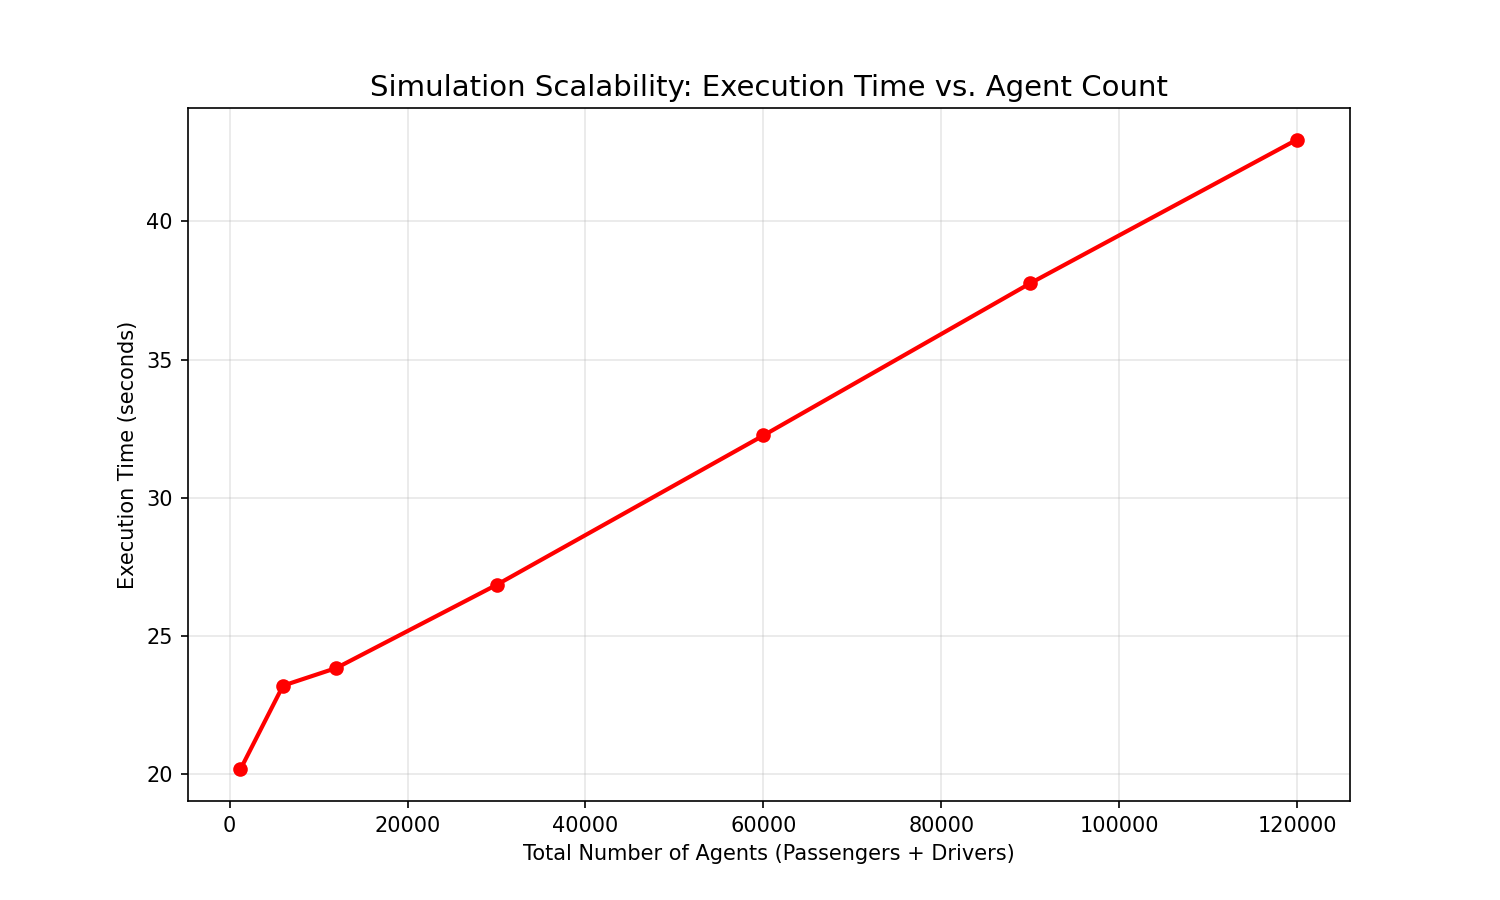
\includegraphics[width=0.7\textwidth]{../plots/idf_analysis/scalability_analysis.png}
    \caption{Simulation Scalability: Execution Time vs. Total Agent Count.}
    \label{fig:scalability}
\end{figure}

\section{Concluding Comments and Perspectives}
Overall, this study introduces a dynamic temporal matching approach to ridesharing that reconciles decentralized user decisions with stable assignment theory. The proposed framework establishes a theoretical basis for modeling sequential matching in transportation systems and opens several avenues for future extensions, particularly toward multi-hop assignments and welfare comparisons with centralized benchmarks.

To fully assess the benefits of ridesharing, congestion should ultimately be modeled endogenously.

We discuss below some limitations of the approach.

\subsection{Limitations of the Current Model}

The main limitations identified are linked to the rigidity of the decision process:

\begin{itemize}

    \item \textbf{Absence of Transfers:}
    The Single-Hop assumption prevents passengers from using multiple successive vehicles.

    This penalizes long-distance trips when no single driver covers the full required path.

    \item \textbf{Early Commitment:}
    The irreversible commitment assumption prevents any renegotiation during the trip.

    A passenger dropped at an intermediate point is forced to complete the remainder of the trip on foot, even if a more advantageous ridesharing opportunity arises afterward.

\end{itemize}

\subsection{Perspective: Multi-Hop Extension}

To overcome these limitations, a natural extension of this work consists in modeling the problem as a \textbf{multi-hop matching problem}. In this framework, the Gale--Shapley algorithm would no longer be applied solely at the initial departure time $t_j^h$, but recursively throughout the trip.

\textbf{Extension Principle:}

Whenever a passenger is dropped off by a first driver $d_1$ at time

$$
t=t_{1,j}^m+tt_{1,j}^c,
$$

they are reintroduced into the active passenger set:

$$
P_{active}(t).
$$

Their new departure time becomes:

$$
t_j^h=t_{1,j}^m+tt_{1,j}^c,
$$

and their origin is updated to their current drop-off location.

Their preference list is then dynamically recomputed for the remaining segment of the trip toward the final destination.

This approach transforms the matching problem into a \textbf{dynamic path-search problem} over a ridesharing opportunity network, opening the way to substantially improved systemic efficiency.

However, this comes at the cost of increased algorithmic complexity and requires more sophisticated management of transfer times and temporal coordination.






\section*{Acknowledgement}
This work was supported by funding from the French National Research Agency (ANR) under the France 2030 program, reference ``ANR-24-PEMO-0003'', project HARMONIC.

\begin{thebibliography}{99}

\bibitem{Agatz2012} Agatz, N., Erera, A., Savelsbergh, M., \& Wang, X. (2012). Optimization for dynamic ride-sharing: A review. \textit{European Journal of Operational Research}, 223(2), 295-303.

\bibitem{Arnott1993} Arnott, R., de Palma, A., \& Lindsey, R. (1993). A Structural Model of Peak-Period Congestion: A Traffic Bottleneck with Elastic Demand. \textit{American Economic Review}, 83(1), 161–179.

\bibitem{Ashlagi2019} Ashlagi, I., Burq, M., Jaillet, P., \& Manshadi, V. (2019). On matching and thickness in heterogeneous dynamic markets. \textit{Operations Research}, 67(4), 927-949.

\bibitem{dePalma2022} de Palma, A., Stokkink, P., \& Geroliminis, N. (2022). Influence of dynamic congestion with scheduling preferences on carpooling matching with heterogeneous users. \textit{Transportation Research Part B: Methodological}, 155, 479-498.

\bibitem{dePalma2024} de Palma, A., Javaudin, L., Stokkink, P., \& Tarpin-Pitre, L. (2024). Ride-sharing with inflexible drivers in the Paris metropolitan area. \textit{Transportation}, 51(3), 963-986.

\bibitem{Furuhata2013} Furuhata, M., Dessouky, M., Ordóñez, F., Brunet, M. E., Wang, X., \& Koenig, S. (2013). Ridesharing: The state-of-the-art and future directions. \textit{Transportation Research Part B: Methodological}, 57, 28-46.

\bibitem{GaleShapley1962} Gale, D., \& Shapley, L. S. (1962). College admissions and the stability of marriage. \textit{The American Mathematical Monthly}, 69(1), 9-15.

\bibitem{Galichon2018} Galichon, A. (2018). \textit{Optimal transport methods in economics}. Princeton University Press.

\bibitem{Kleiner2011} Kleiner, A., Nebel, B., \& Ziparo, V. A. (2011). A mechanism for dynamic ride sharing based on parallel auctions. \textit{Proceedings of the Twenty-Second International Joint Conference on Artificial Intelligence}, 266–272.

\bibitem{Masson2014} Masson, R., Lehuédé, F., \& Péton, O. (2014). The dial-a-ride problem with transfers. \textit{Computers \& Operations Research}, 41, 12-23.

\bibitem{Roth1990} Roth, A., \& Sotomayor, M. A. O. (1990). \textit{Two-sided matching: study in game-theoretic modeling and analysis}. Cambridge University Press.

\bibitem{Small2024} Small, K. A., Verhoef, E. T., \& Lindsey, R. (2024). \textit{The economics of urban transportation}. Routledge.

\bibitem{Stiglic2015} Stiglic, M., Agatz, N., Savelsbergh, M., \& Gradisar, M. (2015). The benefits of meeting points in ride-sharing systems. \textit{Transportation Research Part B: Methodological}, 82, 36-53.

\bibitem{Stokkink2025} Stokkink, P., de Palma, A., \& Geroliminis, N. (2025). Optimizing multi-modal ride-matching with transfers. \textit{Transportation Research Part C: Emerging Technologies}, 179, 105274.

\end{thebibliography}

\end{document}

